\label{apx:tait_colourings}
In this appendix we will discuss a very old theorem first proposed by Scottish physicist Peter Tait, who in the late 1800s was working towards a proof of the four-colour theorem. In his attempt to simplify the problem, Tait found a correspondence between the problem of four-colouring the faces of a graph and three-colouring the edges~\cite{tait_remarks_1880, appel_every_1989}. Tait used this result to construct an incorrect proof of the four-colour theorem, which stood unchallenged for 11 years until a counterexample was provided by Julius Petersen~\cite{petersen_theorie_1891,mulder_julius_1992}. Here we will provide a simple proof of Tait's original correspondence, which states that:

\textbf{Every bridge-free cubic planar graph can be face-coloured with four colours if and only if it can be edge-coloured with 3 colours.}

Let us start by making a few definitions. We will be working only with fully connected cubic graphs, consisting of a set of vertices $v_i$, edges $e_i$ and faces $f_i$ -- where every vertex connects to three edges. Furthermore, a bridge is an edge where, if it were removed the graph would be divided into two connected components. For example in the following graph, the red edge is a bridge, so the graph is considered illegal.
\begin{center}
    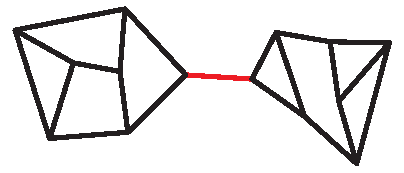
\includegraphics{appendices/figures/bridge.pdf}
\end{center}
Let us construct a labelling system for our faces and edges. Rather than using an integer from 0-4, we will label them using a binary representation of these integers, 
\begin{align}
    \mathfrak l \in \textup{IF}^2_2 = \{ (0,0), \ (0,1), \ (1,0),\ (1,1)\},
\end{align}
where $\textup{IF}^2_2$ is a 2d vector space over the finite field of order 2. Note we always denote a label with $\mathfrak{fraktur}$. On this space, let us define a `subtraction' operator as the bitwise XOR of two labels. Note that this operator is associative, commutative, and has an identity element which we label $\textbf 0 = (0,0)$. We refer to this as a `subtraction' because it satisfies the following property
\begin{align}
    \mathfrak l_1 \oplus \mathfrak l_2 = (0,0) \implies \mathfrak l_1 = \mathfrak l_2,
\end{align}
although it does fail to satisfy some other properties one might expect of subtraction such as having $\mathfrak l_1 \oplus \mathfrak l_2 = \mathfrak l_2 \oplus \mathfrak l_1$.

We shall define a 4-face colouring by assigning one of these four labels $\mathfrak f$ to each of the faces in the graph, with the condition that no two adjacent faces share the same label. 
\begin{align}
    \mathfrak{f}: f_i\rightarrow \mathfrak{f}_i \in \textup{IF}^2_2
\end{align}
Similarly, we define a 3-edge colouring by assigning an edge label $\mathfrak e$ from the three nonzero labels such that no vertex touches two edges with the same label. 
\begin{align}
    \mathfrak{e}: e_i\rightarrow \mathfrak{e}_i \in  \textup{IF}^2_2 / \textbf 0
\end{align}

Now let us suppose that we have two labelled faces, $f_1$ and $f_2$, which are separated by an edge $e$. We assert that a valid edge colouring can be found by taking the difference of the two adjacent face colours
\begin{align} \label{eqn:face_to_edge}
    \mathfrak e = \mathfrak f_1 \oplus \mathfrak f_2.
\end{align} 

Thus, we may visualise the face colours as behaving something like a `height' or `position' coordinate, and the edge colours as acting more like a `difference' coordinate. Now let us prove that the relation above provides a direct mapping from any valid 4-face colouring to a 3-edge colouring and vice versa, see Fig.~\ref{fig:face_edge_colouring}.

\begin{figure}[t]
    \centering
    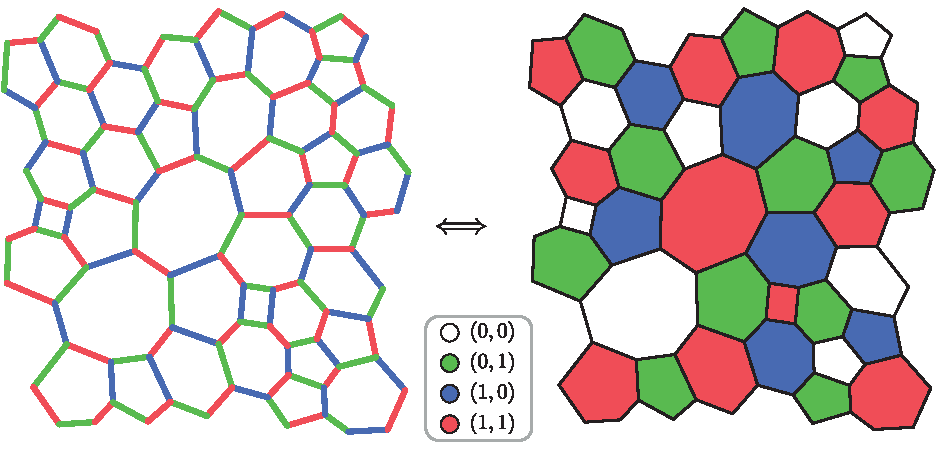
\includegraphics[width=0.9\textwidth]{appendices/figures/four_colouring.pdf}
    \caption[A 3-edge colouring on a tri-coordinated graph, transformed into a valid 4-colouring of the faces.]{ An example of a 3-edge colouring on a graph with coordination number $z\leq3$, along with the corresponding 4-face colouring, related according to Eqn.~\ref{eqn:face_to_edge}. }
    \label{fig:face_edge_colouring}
\end{figure}%

\section{4-Face Colouring to a 3-Edge Colouring}

Suppose we start with a valid 4-face colouring. Let us show that the relation in Eqn.~\ref{eqn:face_to_edge} always allows us to transform this into a valid edge colouring. Firstly, note that, provided that no adjacent faces have the same colour, we are guaranteed to have only three colours in our edge colouring. This is because an edge will only have colour $\textbf 0$ if the two faces it borders have the same colour, however this is prohibited for the face colouring to be valid. 

Now we must show that it is not possible for any vertex to touch two edges of the same colour. Let us consider a single vertex between three faces. Each face has a distinct colour $\mathfrak f_i$ and each edge that meets this vertex has a colouring $\mathfrak e_i$ as shown below:
\begin{center}
    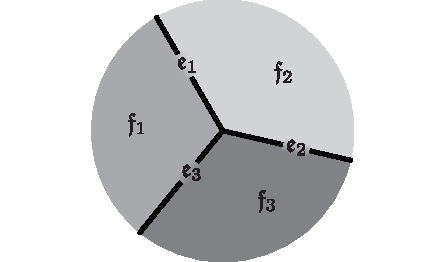
\includegraphics{appendices/figures/site_e_f.pdf}
\end{center}
Now let us consider the quantity
\begin{align} \label{eqn:e_i_sum}
    \mathfrak m = \mathfrak e_1 \oplus \mathfrak e_2 \oplus \mathfrak e_3
\end{align}
Using Eqn.~\ref{eqn:face_to_edge} we may rewrite this in terms of the face colours as
\begin{align} 
    \begin{aligned}
    \mathfrak m &= (\mathfrak f_1 \oplus \mathfrak f_2) \oplus (\mathfrak f_2 \oplus \mathfrak f_3) \oplus(\mathfrak f_3 \oplus \mathfrak f_1) = \textbf 0,
    \end{aligned}
\end{align}
since every term appears twice in this sum. No edge can have $\mathfrak e_i = \textbf 0$, so the only way for $\mathfrak e_i$ to satisfy Eqn.~\ref{eqn:e_i_sum} is to have one $\mathfrak e_i$ of each nonzero type. Thus, we see that $\mathfrak e_i$ represents a valid edge colouring around the vertex. In general this means that a valid face colouring will always generate a valid face colouring.

\section{3-Edge Colouring to a 4-Face Colouring} \label{sec:edge_to_face}

Suppose we start with a valid 3-edge colouring and are instructed to transform it into a valid 4-face colouring. To do this, let us pick an arbitrary face of the graph -- labelled $f_0$ -- and assign it an arbitrary colour, say $(0,0)$. Now, given an arbitrary face, $f_j$, we may determine its colour $\mathfrak{f}_j$ by traversing from $f_0$ to $f_j$, and  taking the sum of the edge colours $\mathfrak e_k$ for every edge that crosses on the path $p$,
\begin{align}\label{eqn:f_path}
    \mathfrak f_j = \mathfrak f_0  \bigoplus_{k \in p} \mathfrak e_k.
\end{align}
The colour of $\mathfrak f_j$ is uniquely defined provided that this process is invariant to the choice of path taken. If we consider two paths $p$ and $p'$, from $f_0$ to $f_j$, shown in Fig.~\ref{fig:two_paths} we require that
\begin{figure}[t]
    \centering
    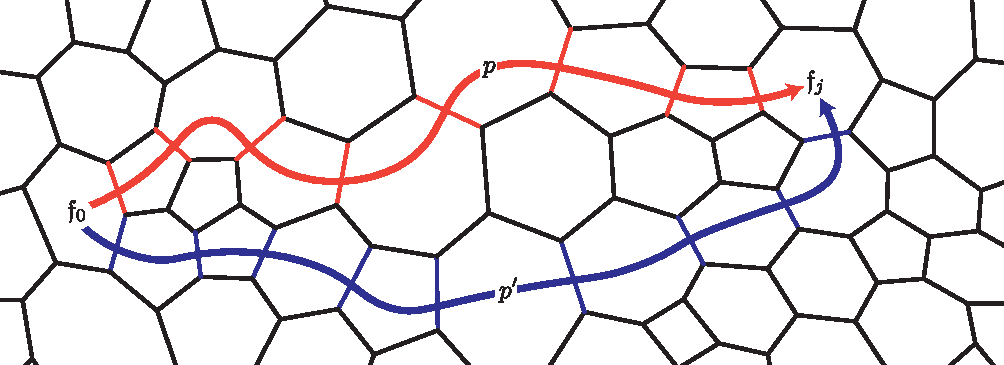
\includegraphics{appendices/figures/f_paths.pdf}
    \caption{Two distinct paths from $f_0$ to $f_j$. The combination of both paths forms a closed loop, where the value of $\mathfrak{f_j}$ is uniquely determined provided that $\bigoplus \mathfrak e$ around this loop vanishes.}
    \label{fig:two_paths}
\end{figure}%
\begin{align}
    \mathfrak f_j = \mathfrak f'_j
    \implies \mathfrak f_j \oplus \mathfrak f'_j = \textbf 0.
\end{align}
Inserting Eqn.~\ref{eqn:f_path} into this expression, we arrive at the condition
\begin{align}
    \textbf 0 = 
    \left ( 
    \bigoplus_{k \in p} \mathfrak e_k 
    \right ) \oplus \left ( 
    \bigoplus_{k \in p'} \mathfrak e_k
    \right )
\end{align}
Since the composition of the two paths is a closed loop, this amounts to the condition that the integral of $\mathfrak e_k$ around any closed loop in the system must vanish.

In order to show this condition holds, let us first notice that -- as we saw in the previous section -- the sum of $\mathfrak e_k$ around any single vertex must vanish if we have a valid 3-edge colouring. Similarly, a path that encloses two vertices is also guaranteed to vanish, since it can be decomposed as a sum of the paths that encircle each vertex individually. Thus, we see that a general closed loop that encircles some set of vertices can always be decomposed into a sum of loops around each individual vertex, which then all vanish individually. 

This argument completes the proof, any path from $f_0$ to $f_j$ will give an identical value for $\mathfrak f_j$. Furthermore, the 4-colouring obtained is guaranteed to always satisfy the condition of no adjacent faces having the same colour, since any two adjacent faces $\mathfrak f_1$ and $\mathfrak f_2$ separated by $\mathfrak e$ must satisfy 
\begin{align}
    \mathfrak f_1 \oplus \mathfrak e = \mathfrak f_2 \neq \mathfrak f_1 \textup{ for } \mathfrak e \neq \textbf 0.
\end{align}

\begin{shaded}
    {\it What about periodic boundaries?} --- 
    The eagle-eyed reader might have noticed an omission in the argument presented. We showed that all closed loops that encircle a set of vertices are guaranteed to have $\bigoplus e = \textbf 0$. However not all closed loops have a defined inside and outside. If we construct such a system on a manifold with genus $g$, then in general there will be $2g$ topologically distinct non-contractible loops. Since these have no inside and outside, the argument above fails, and it is possible for such non-contractible loops to have $\bigoplus e \neq \textbf 0$. In such a case, a valid 3-edge colouring does not imply a 4-face colouring. 

    Thus, on a manifold that is not simply connected, a 4-face colouring implies a 3-edge colouring however a 3-edge colouring \textit{does not} imply a 4-face colouring!
\end{shaded}

% \section{The Four-Unit-Cell Spin Transformation}
% Here we show that the four unit four-unit-cell transformation presented in \textsection\ref{sec:spin_flip_transformation} is precisely equivalent to this argument. However here, rather than connecting a 3-edge colouring to a 4-face colouring, we connect it to a 4-vertex colouring. Let us start by restating the problem in a rather more abstract way than that presented in \textsection\ref{sec:spin_flip_transformation}.